This section shows how the components run and interact in the system, by using Sequence Diagrams.

\subsubsection{Application Opening}

	\begin{figure}[H]
		\centering
		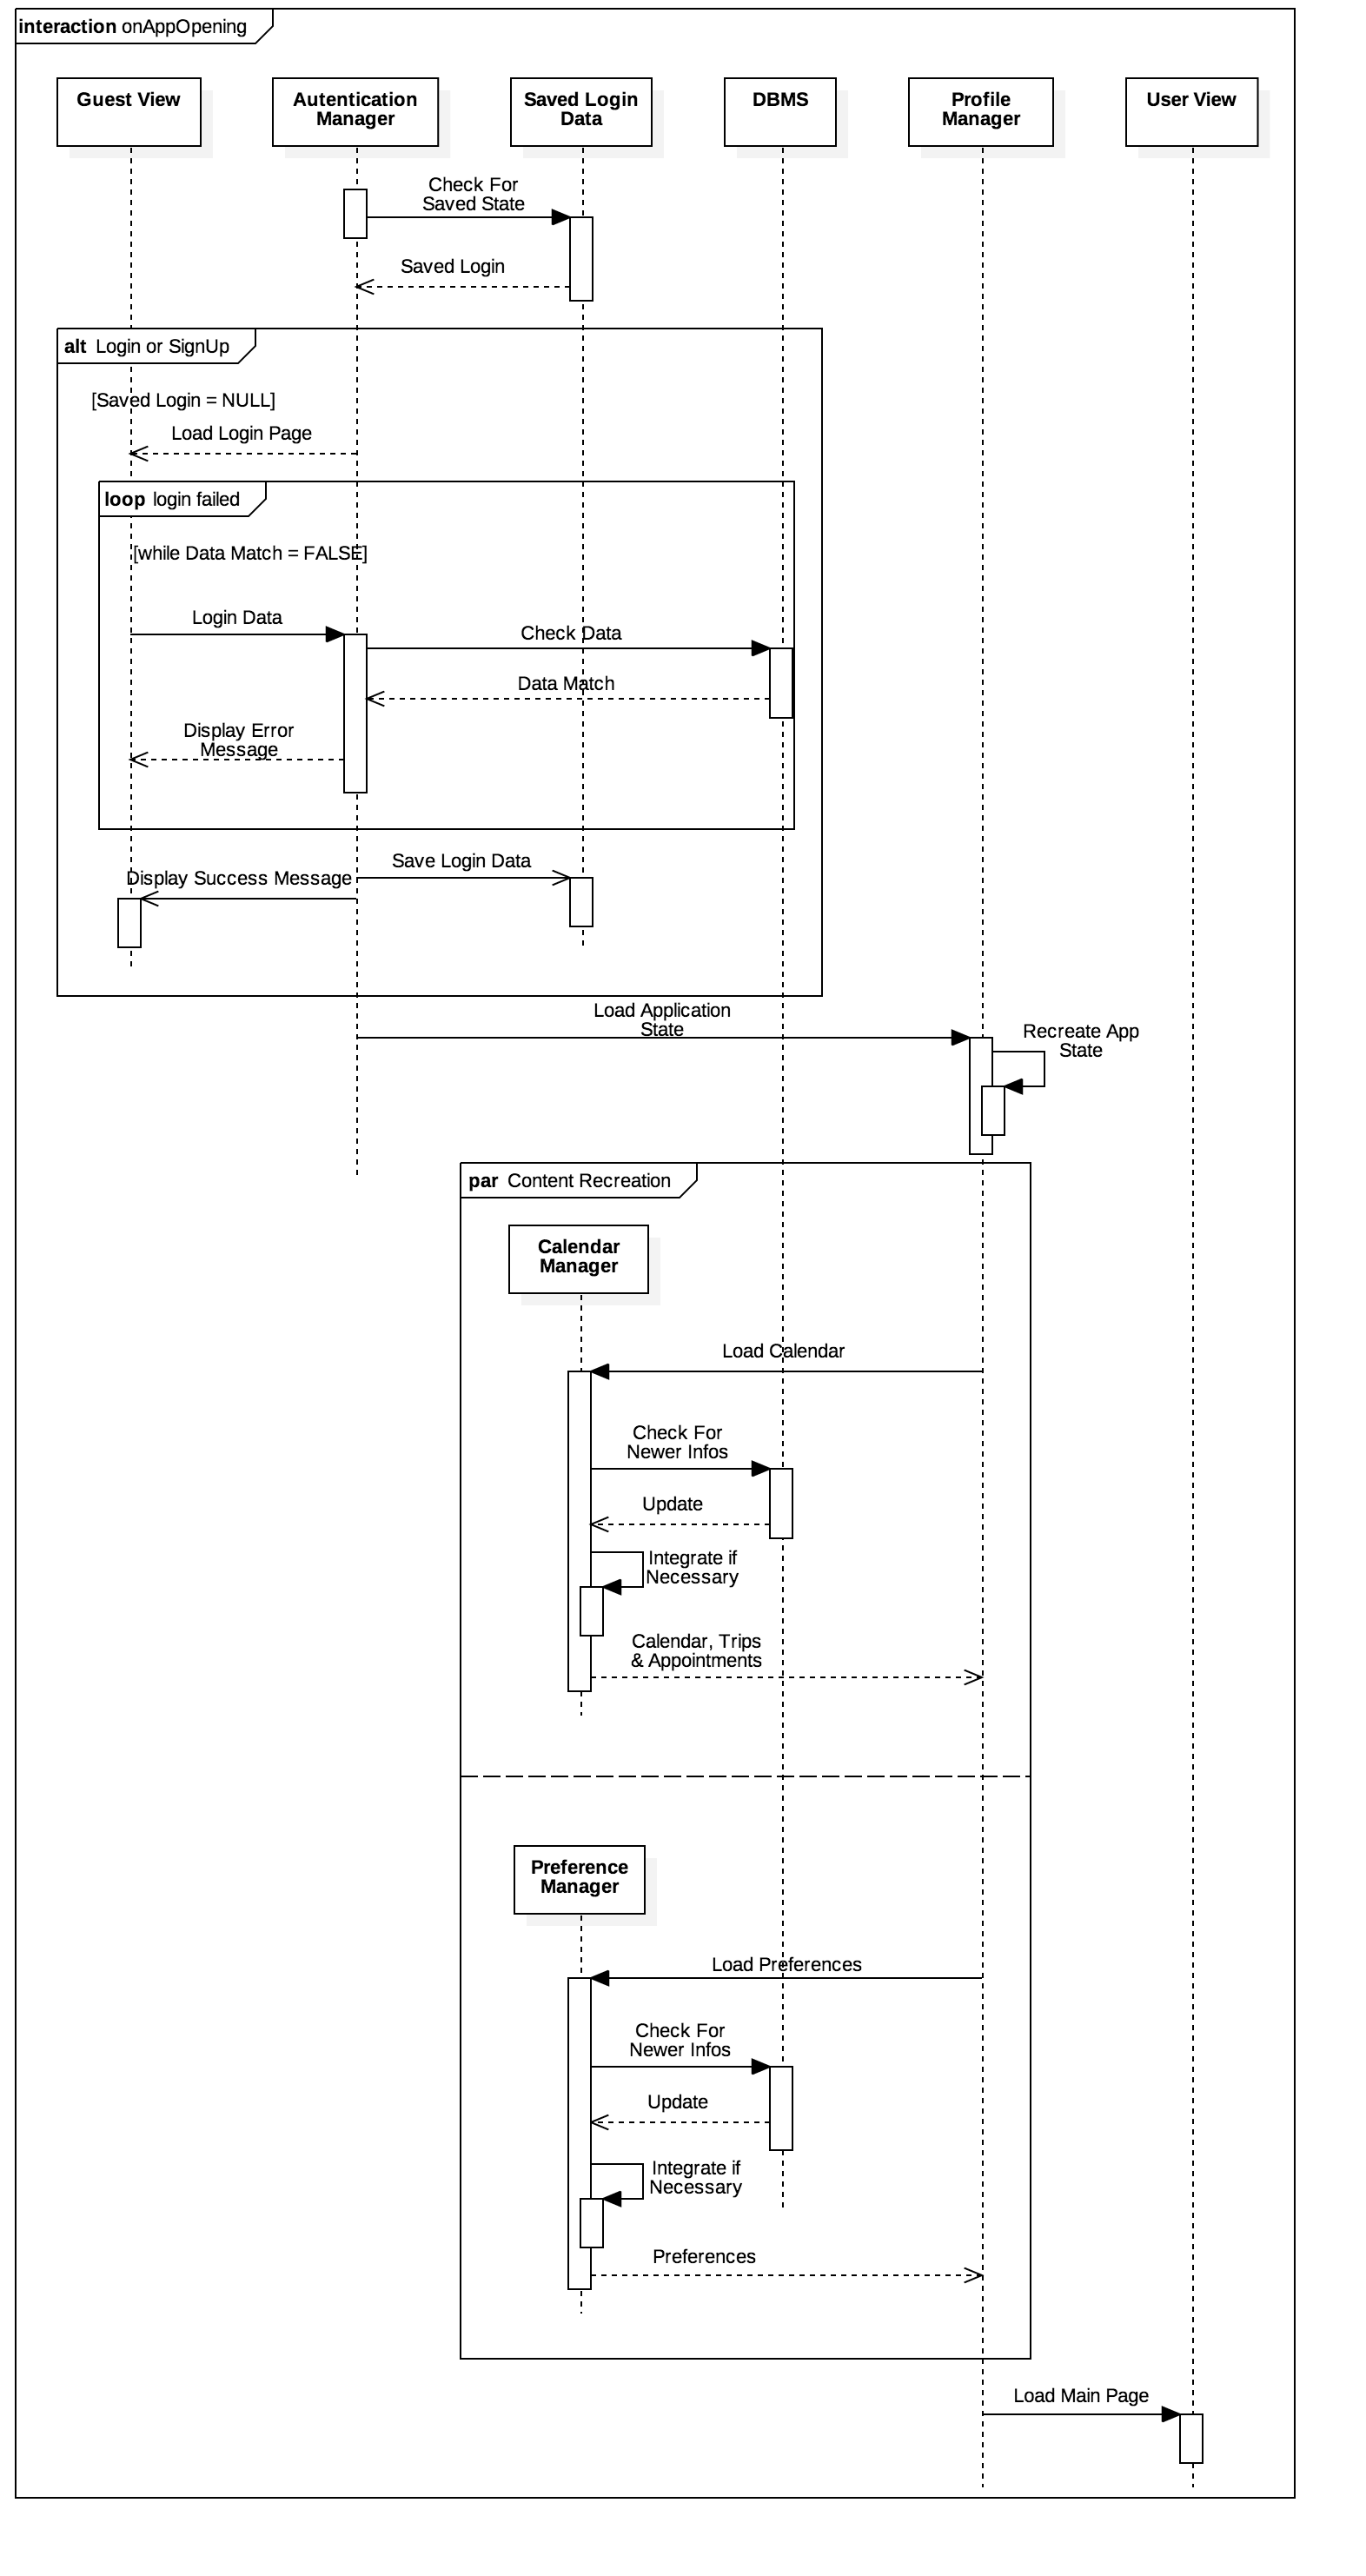
\includegraphics[width=\textwidth]{UML/runtimeView/onAppOpening}
		\caption{Login Sequence Diagram}
		\label{loginRunTimeView}
	\end{figure}
	
	This Sequence Diagram represents the first operations of \textit{Travlendar+}.
	When application is opened, the \textsl{Auto Login} Procedure in the 'Access Manager' (see figure \ref{accessManagerDetail}) takes place: the 'Autentication Manager' checks for 'previously accesses data' in 'Saved Data Login' component. If the User has logged before, the User View is logged as explained later.
	On the contrary the \textsl{Login Page} of 'Guest View' of 'Mobile Application' component  (see figure \ref{mobileApplicationDetail}) is loaded.
	
	On this page the User, if already registered, he must fill the login form with his credential.
	'Autentication Manager' connects then to the 'DMBS' in the  '\textit{Travlendar} Server' component (see figure \ref{serverDetail}) in order to check if the form is properly compiled.
	
	'DBMS' returns a Result; if the credential are correct 'Autentication Manager' notifies Guest of the success of the procedure, and saves the aforementioned data to the 'Saved Data Login' component.
	
	Then a the \textsl{Content Recreation} procedure starts:
	'Profile Manager' in 'Application Aggregator' component (see figure \ref{applicationAggregatorDetail}) loads all the necessary information about the User, and makes 'Calendar Manager' load all the informations about Appointments, Trips, and Breaks of the User; if necessary, 'Calendar Manager' and 'Preference Manager' (see figure \ref{preferenceManagerDetail}) have to restore them from the 'DBMS'.
	After all the data are loaded, the component 'User View' in 'Mobile Application' is told to show the \textsl{MainPage} to the User.
	
	In case of incorrect credentials, 'Autentication Manager' make the 'Guest View' notify the User of the not well compiled form, and makes him try again until the insertion of correct credentials.
	
	
\subsubsection{Event Solutions Refreshing}

	\begin{figure}[H]
		\centering
		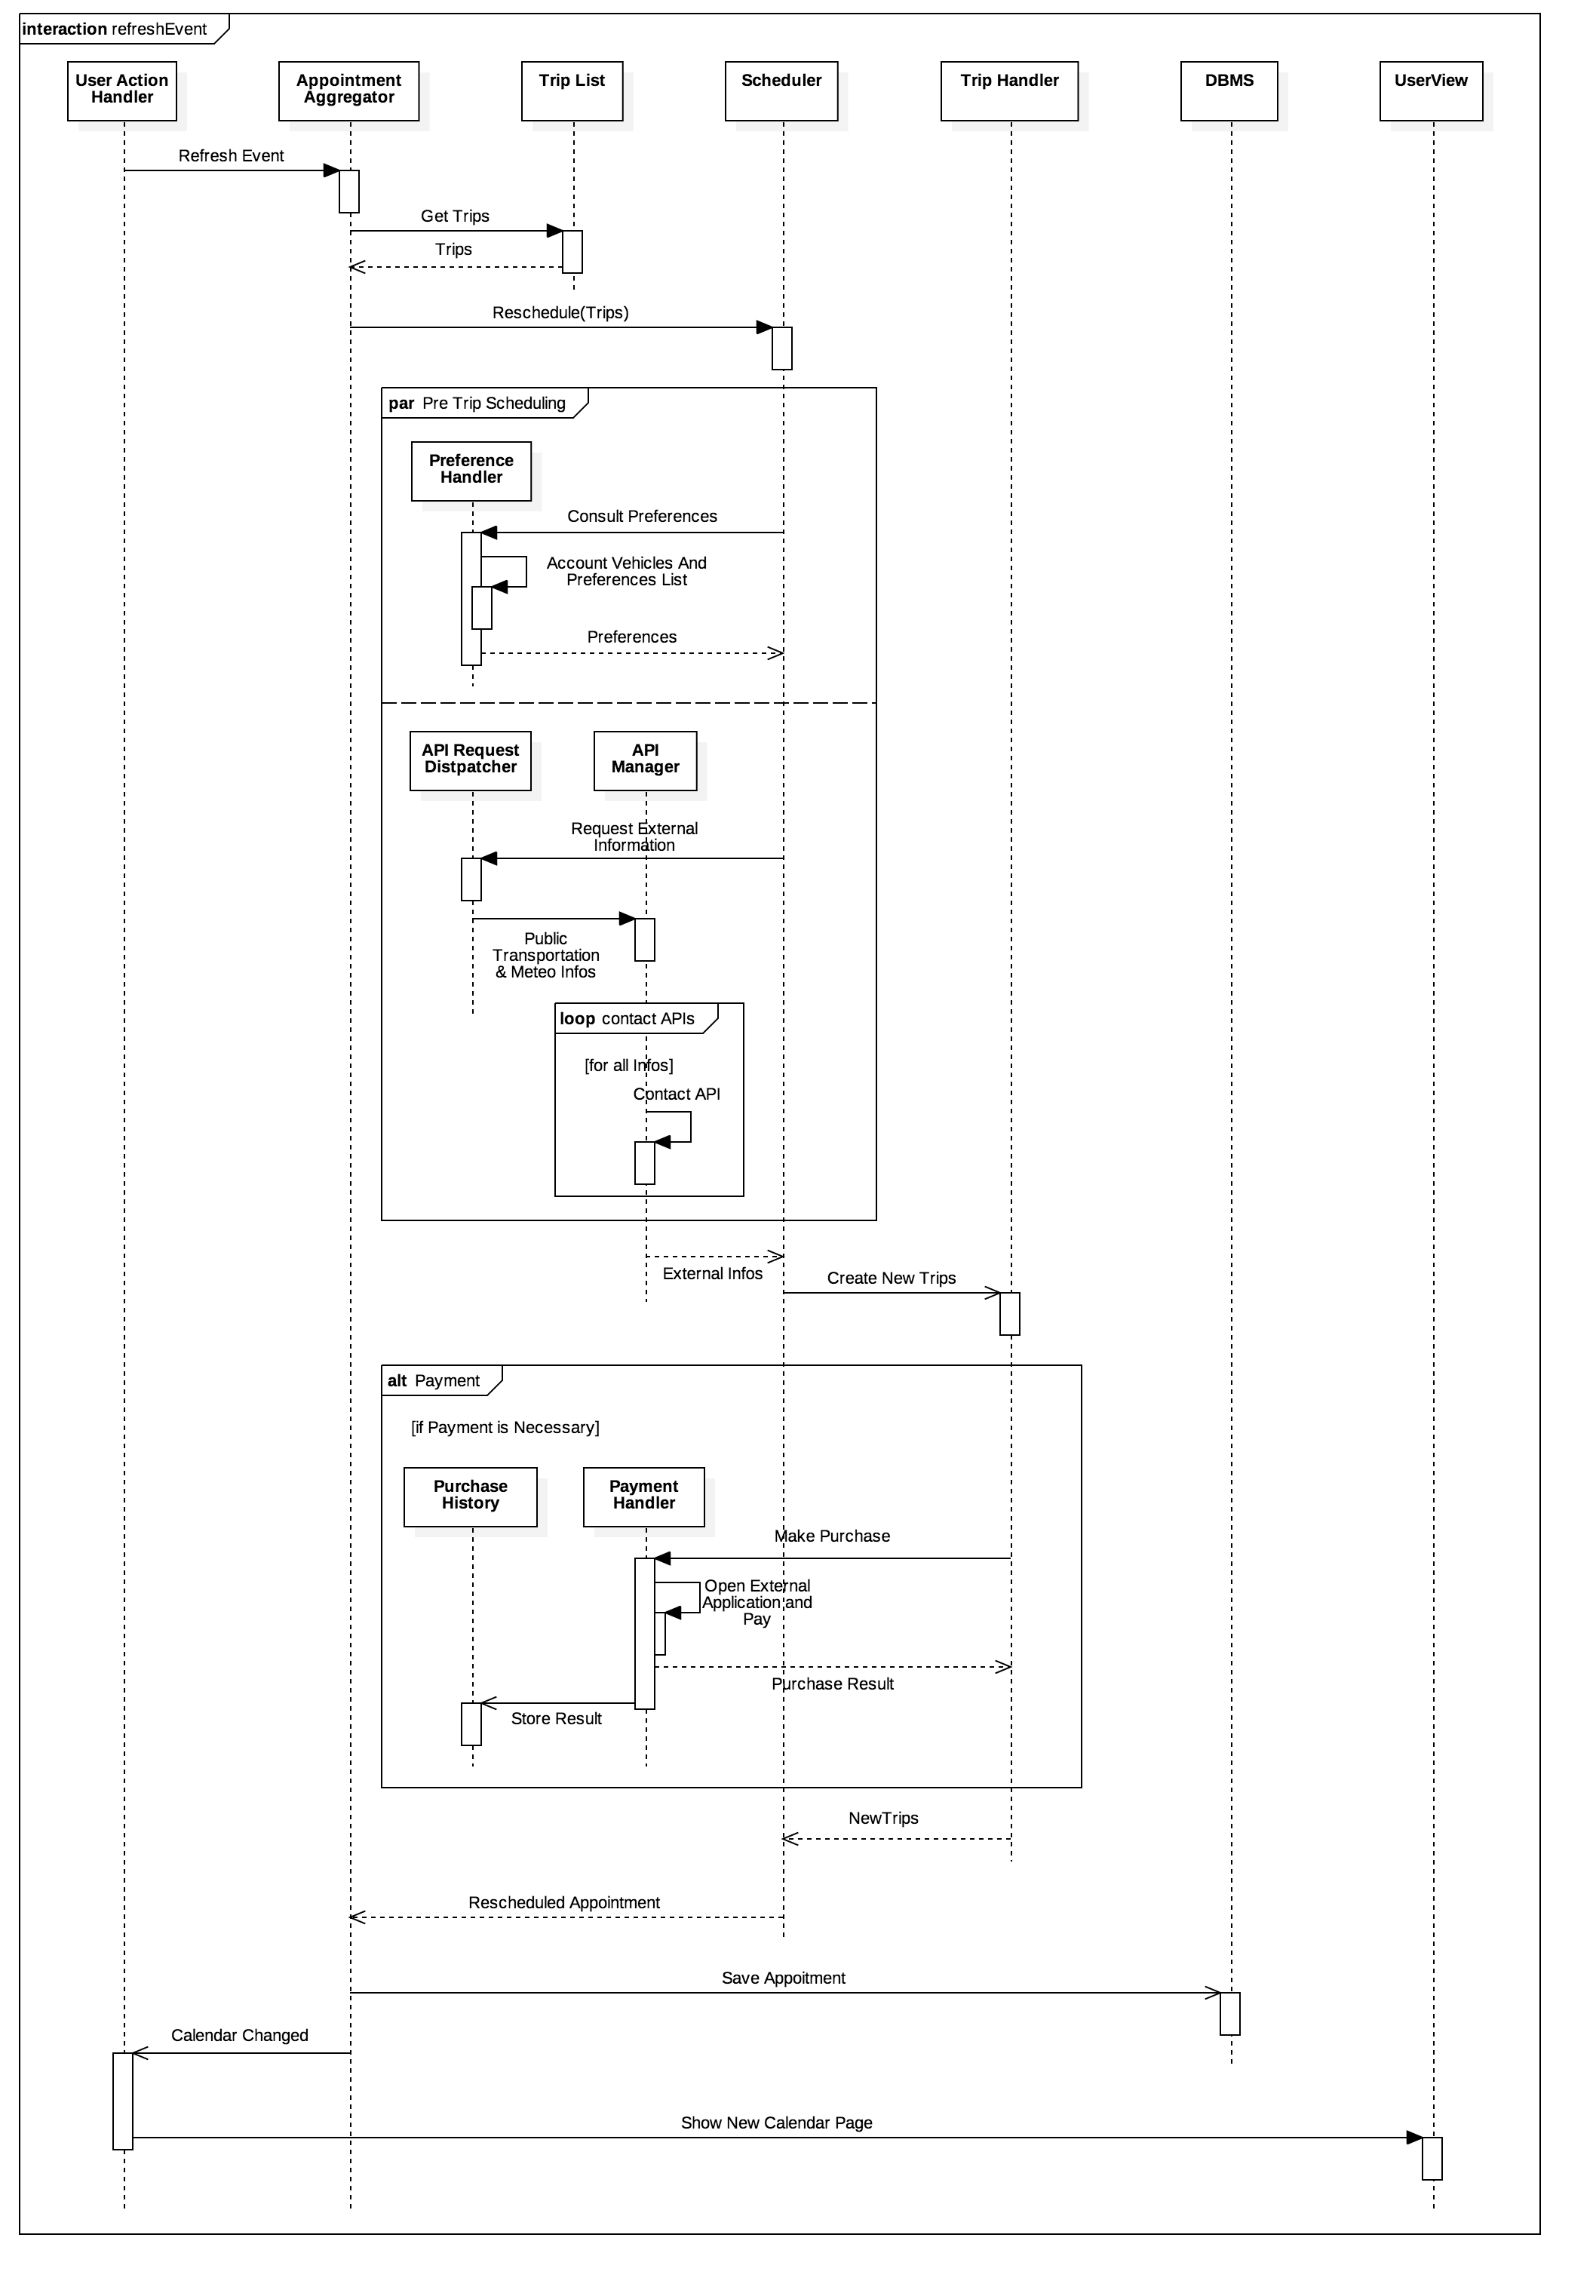
\includegraphics[width=0.9\textwidth]{UML/runtimeView/refreshEvent}
		\caption{Login Sequence Diagram}
		\label{refreshRunTimeView}
	\end{figure}